\documentclass{article}

% if you need to pass options to natbib, use, e.g.:
\PassOptionsToPackage{numbers, compress}{natbib}
% before loading nips_2017
%
% to avoid loading the natbib package, add option nonatbib:
% \usepackage[nonatbib]{nips_2017}

\usepackage[final]{nips_2017}


%\usepackage[square,numbers]{natbib}
\bibliographystyle{abbrvnat}


\usepackage[utf8]{inputenc} % allow utf-8 input
\usepackage[T1]{fontenc}    % use 8-bit T1 fonts
\usepackage{hyperref}       % hyperlinks
\usepackage{url}            % simple URL typesetting
\usepackage{booktabs}       % professional-quality tables
\usepackage{amsfonts}       % blackboard math symbols
\usepackage{nicefrac}       % compact symbols for 1/2, etc.
\usepackage{microtype}      % microtypography
\usepackage{subcaption}
\usepackage{graphicx}

% Choose a title for your submission
\title{Story Cloze Test}


\author{Lea Fritschi \qquad Beat Hubmann \qquad  Maya V\"ogeli \qquad   Lukas Wampfler}

\begin{document}
% \nipsfinalcopy is no longer used

\maketitle

% We do not require you to write an abstract. Still, if you feel like it, please do so.
%\begin{abstract}
%\end{abstract}
\section{Introduction}
You can keep this short. Ideally you introduce the task already in a way that highlights the difficulties  your method will tackle.
\section{Methodology}

In our approach we use the idea of {\bf quick thoughts}, as proposed in \cite{eff_framework}. The basic idea is to train an encoder in order to learn an embedding for the four context sentences (the first four sentences of the short story). Instead of using a decoder, the model then uses a classifier to identify the correct sentence from the set of two candidate sentences (basically deciding which of the two candidate embeddings is closer to the embedding of the four starting sentences of the story.\\[.1cm]
Is there a particular additional data source you want to use? \\[.1cm]
{\bf Frage: } Wurde anderer Code (zB von \cite{eff_framework}) verwendet? Falls ja, sollte man das deklarieren.
\section{Model}
We use the meaning of the first four sentences to predict the meaning of the last sentence, where meaning is represented by an embedding of the context computed from an encoding function. Our loss function is defined in feature space. \\[.1cm]
Formally: Let $f$ and $g$ be parametrized functions that take a context of four sentences ($f$) resp. a single sentence ($g$) as input and encode it into a fixed length vector of equal size. For a given candidate sentence $s_{cand}$ and the set $S_{cand}$ of all possible candidate sentences (two in our case), the probability that $s_{cand}$ is the correct last sentence, is given by 
$$
p(s_{cand} | \, cont, S_{cand}) = \frac{exp(c(f(cont), g(s_{cand})}{\sum_{s' \in S_{cand}}exp(c(f(cont), g(s')}
$$
where $cont$ denotes the four-sentence context of the last sentence and $c$ is a scoring function/ classifier. {\bf comment: this is taken from \cite{eff_framework}: is this correct?}
\\[.1cm]
For the encoder, we used a bidirectional RNN with 600 GRU-cells. \\[.1cm]
Attention mechanism ? Gibt es dazu etwas zu sagen?
{\bf Image of architecture:}
\begin{figure}[h]
\begin{subfigure}[c]{0.5\textwidth}

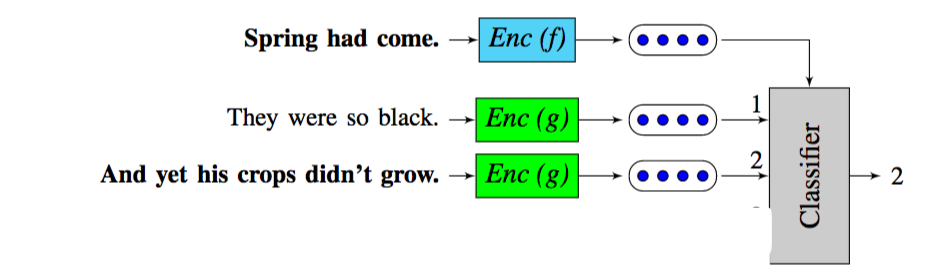
\includegraphics[width=0.9\textwidth]{fig1_architecture}
\subcaption{Figure taken from \cite{eff_framework}}

\end{subfigure}
\begin{subfigure}[c]{0.4\textwidth}

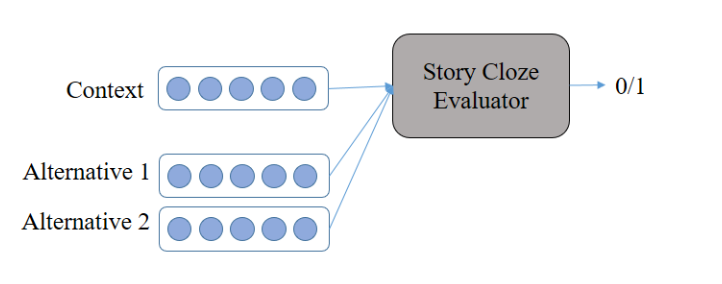
\includegraphics[width=0.9\textwidth]{fig2_architecture}
\subcaption{Figure taken from \cite{mostafazadeh-EtAl:2016:RepEval}}

\end{subfigure}
\caption{{\bf Frage: }Welche Art von Grafik ist für den Report geeigneter (links: m\"usste ich noch anpassen auf unsere Methode; die Grafik rechts k\"onnte man so \"ubernehmen.}
\end{figure}



\section{Training}
For training, we used a corpus of $88161$ five sentence stories. In these stories, there were no alternative (wrong) ending sentences. 
We used GloVe pretrained word embeddings in 300 dimensions.\cite{pennington2014glove}. \\[.1cm]
The training objective maximizes the probability .... (to be continued)

What is your objective? How do you optimize it?

\section{Experiments}
On the validation set, we achieve an accuracy of $0.60$. This result is comparable with respect to what has been published earlier \cite{}
This {\bf must} at least include the accuracy of your method on the validation set.
\section{Conclusion}
You can keep this short, too.

%\bibliographystyle{plain}
\bibliography{bibliography} 
\end{document}
